\documentclass[12pt]{report}

% ====================== PACKAGES ======================
\usepackage[french]{babel} % French language support
\usepackage[utf8]{inputenc} % UTF-8 encoding
\usepackage[T1]{fontenc} % Character encoding
\usepackage{amsmath, amssymb, amsfonts} % Math packages
\usepackage{graphicx} % Required for inserting images
\usepackage{float} % Improved handling of floating elements
\usepackage{hyperref} % For hyperlinks
\usepackage{array, tabularx, multirow, multicol} % Table packages
\usepackage{caption, subcaption} % Caption and subcaption for figures and tables
\usepackage{setspace} % Set line spacing
\usepackage{abstract} % Abstract layout
\usepackage{color, xcolor} % Color handling
\usepackage{lipsum} % For generating filler text
\usepackage{fancyhdr} % Fancy headers and footers
\usepackage{titlesec} % Section formatting
\usepackage{enumerate} % Enumerate with custom labels
\usepackage{booktabs, colortbl} % Improved table formatting
\usepackage{geometry} % To define page margins
\usepackage{longtable} % For tables spanning multiple pages
\usepackage{listings}
\usepackage{bm}

% ====================== COMMANDS ======================
\providecommand{\abs}[1]{\lvert#1\rvert} % Absolute value command
\DeclareMathOperator{\sign}{sign} % Sign function

% ====================== PAGE GEOMETRY ======================
\geometry{top=2cm, bottom=3cm, left=2cm, right=2cm} % Adjust top margin to provide space for header
\setlength{\headheight}{45pt} % Increase headheight to fit header content
\setlength{\headsep}{20pt} % Add space between header and text

% ====================== PDF METADATA ======================
\hypersetup{ % Information about the PDF document
    pdfauthor = {Premier Auteur}, % Authors
    pdftitle = {Nom du Projet - Sujet du Projet}, % Title
    pdfsubject = {Mémoire de Projet}, % Subject
    pdfkeywords = {Tag1, Tag2, Tag3}, % Keywords
    pdfstartview={FitH}, % Adjust page width to screen width
    colorlinks=true, % Colored links
    citecolor=black, % Citation links color
    filecolor=black, % File links color
    linkcolor=black, % Internal links color
    urlcolor=black % URL links color
}

\lstset{
    language=Python,
    basicstyle=\ttfamily\footnotesize,
    keywordstyle=\color{blue},
    commentstyle=\color{orange},
    stringstyle=\color{red},
    showstringspaces=false,
    numberstyle=\tiny\color{gray},
    numbers=left,
    stepnumber=1,
    numbersep=5pt,
    frame=single,
    breaklines=true,
    backgroundcolor=\color{lightgray},
    captionpos=b,
    tabsize=4,
    morekeywords={Material, self},
}

\lstdefinelanguage{Faust}{
  keywords={import, process, os.osc, hslider},
  keywordstyle=\color{blue}\bfseries,
  sensitive=true,
  comment=[l]{//},
  morecomment=[s]{/*}{*/},
  commentstyle=\color{gray}\itshape,
  stringstyle=\color{red},
  morestring=[b]",
}

% ====================== HEADER AND FOOTER ======================
\pagestyle{fancy} % Enable fancy headers and footers
\fancyhf{} % Clear all header and footer fields

\fancyhead[L]{ % Left header
    \begin{minipage}{1.5cm}
        \centering
        
\includegraphics[width=0.80\textwidth]{imgs/LogoCN_Q.pdf}
    \end{minipage}
    \begin{minipage}{12cm}
        \small \textsc{École}\\
        \small \textsc{Centrale}\\
        \small \textsc{Nantes}\\
    \end{minipage}
}
\fancyhead[R]{ % Right header
    \begin{minipage}{4.8cm}
        \raggedleft
        \small \textsc{stage vision}\\
    \end{minipage}
}
\fancyfoot[R]{\large \textbf{\thepage}} % Right footer with page number

\renewcommand{\headrulewidth}{0.2pt} % Header rule width
\renewcommand{\footrulewidth}{0.2pt} % Footer rule width

% ====================== SECTION FORMATTING ======================
\titleformat{\chapter}[display]
    {\normalfont\bfseries}{}{0pt}{\Large}
\titlespacing*{\chapter}{0pt}{-20pt}{20pt}

% ====================== BEGIN DOCUMENT ======================
\begin{document}
\pagenumbering{arabic} % Start page numbering in arabic numerals
\renewcommand{\labelenumii}{\arabic{enumi}.\arabic{enumii}}

% Title page
\begin{titlepage}
    \centering
    \vspace*{0cm}
    
\includegraphics[width=0.3\textwidth]{imgs/LogoCN_Q.pdf}
    
    \vspace{3cm}
    
    \Huge\textbf{Rapport TP : MUNUM}\\
    \vspace{1cm}
    \Large\textbf{}\\
    
    \vspace{2cm}
    \Large\textbf{Synthèse sonore musicale avec FAUST}\\
    
    \vfill
    
    \Large{Viozelange Matis}\\
    \vspace{0.5cm}
    
    \vfill

    \vspace{2cm}
    
    \Large\textit{date : \today}\\
    
    \vspace{0.5cm}
    
    \Large\textbf{École Centrale Nantes}\\
    
    \vspace*{1cm}
\end{titlepage}


\newpage
\thispagestyle{empty}
~

\chapter{PARTIE 1 : Synthèse additive}

\section{Contrôle du volume et de la fréquence}

Code pour régler fréquence et amplitude :

\begin{lstlisting}[language=Faust]
    import("stdfaust.lib");
    process = os.osc(frequency) * gain;
    gain = hslider("gain", 0.1, 0, 1, 0.01);
    frequency = hslider("freq", 440, 0, 20000, 1);
\end{lstlisting}

\section{Envelope temporelle}

\begin{lstlisting}[language=Faust]
    gate = button("gate");
    profile = en.ar(0.002, 0.1);
    envelope = gate : profile;
    process = os.osc(440) * envelope;
\end{lstlisting}

La ligne profile du code ci-dessus crée un profil d'attaque de 0.002s et de relâchement de 0.1s. % 
L'enveloppe associe le profil au bouton \textit{gate}.

En contrôlant les gains du profil avec le code ci-dessous, on peut obtenir un son %
percussif avec un petit temps d'attaque et un son avec du \textit{sustain} en allongeant l'attaque %
et le relâchement.

\begin{lstlisting}[language=Faust]
    gate = button("gate");
    profile = en.ar(0.002 * attack, 0.1 * release);
    envelope = gate : profile;

    attack = hslider("attack", 1, 0, 100, 0.1);
    release = hslider("release", 1, 0, 10, 0.01);

    process = os.osc(440) * envelope;
\end{lstlisting}

\section{Harmonic additive model}
On analyse l'influence des harmoniques de ce code : 

\begin{lstlisting}[language=Faust]
    import("stdfaust.lib");

    partialslider(n) = hslider("partial %n", 0.25, 0, 1, 0.01);
    partial(n,f) = os.osc(f*n) * partialslider(n);
    freqslider = hslider("freq", 200, 100, 800, 1);
    process = sum(i, 4, partial(i+1, freqslider));
\end{lstlisting}

On remarque que la hauteur d'une note n'est pas influencée par l'absence du fondamental. % 
Cependant, si on atténue les fréquences impaires (1 et 3), la note semble monter d'une octave. % 

Augmenter n ne change pas la hauteur de la note mais son timbre. De manière %
générale, jouer sur les harmoniques change d'abord le timbre %
d'une note comme l'a si bien remarqué Rousseau.

\chapter{PARTIE 2 : Synthèse soustractive}

\section{Écho}
\begin{lstlisting}[language=Faust]
    bounce = @(4410 * slider) : *(0.75);
    slider = hslider("gain", 1, 0, 10, 0.02);
    echo = +~bounce;
    process = echo;
\end{lstlisting}

Le code ci-dessus crée un effet d'écho sur un signal d'entrée. Le terme \textit{@(4410 * slider)} sert %
à choisir la fréquence de l'écho en jouant sur le retard des signaux en écho.

L'opérateur "~" sert à donner un feedback à l'entrée de la boucle. Le terme de retour est simplement %
le signal de sortie, ce qui crée cet effet d'écho.

\section{Algorithme de Karplus-Strong}

On implémente le code ci-dessous : 

\begin{lstlisting}[language=Faust]
    import("stdfaust.lib");
    mean(x) = (x+x')/2;
    delayslider = hslider("delay", 0, 0, 200, 1);
    gainslider = hslider("gain", 0, -0.98, 0.98, 0.01);
    feedback = @(delayslider) : mean : *(gainslider);
    noiseslider = hslider("noise", 0.5, 0, 1, 0.01);
    process = no.noise * noiseslider : + ~ feedback;
\end{lstlisting}

La fonction \textit{mean} joue le rôle d'un filtre passe-bas en faisant la moyenne entre x et x', où x' est x pris % 
à un instant précédent et proche. Le feedback permet de distribuer l'énergie du bruit sur les fréquences %
cibles pour synthétiser le son voulu.
Plus le gain tend vers 1, plus le son passe du bruit à un signal harmonique. 
Le délai quant à lui joue sur la hauteur du son perçu.

\section{Synthèse d'une guitare}

Pour la synthèse de la guitare, on ajoute une enveloppe avec le code vu ci-dessus pour le réalisme et on % 
pousse le gain très proche de 1. On obtient les réglages figure \ref{fig:guitar}.

\begin{figure}
    \centering
    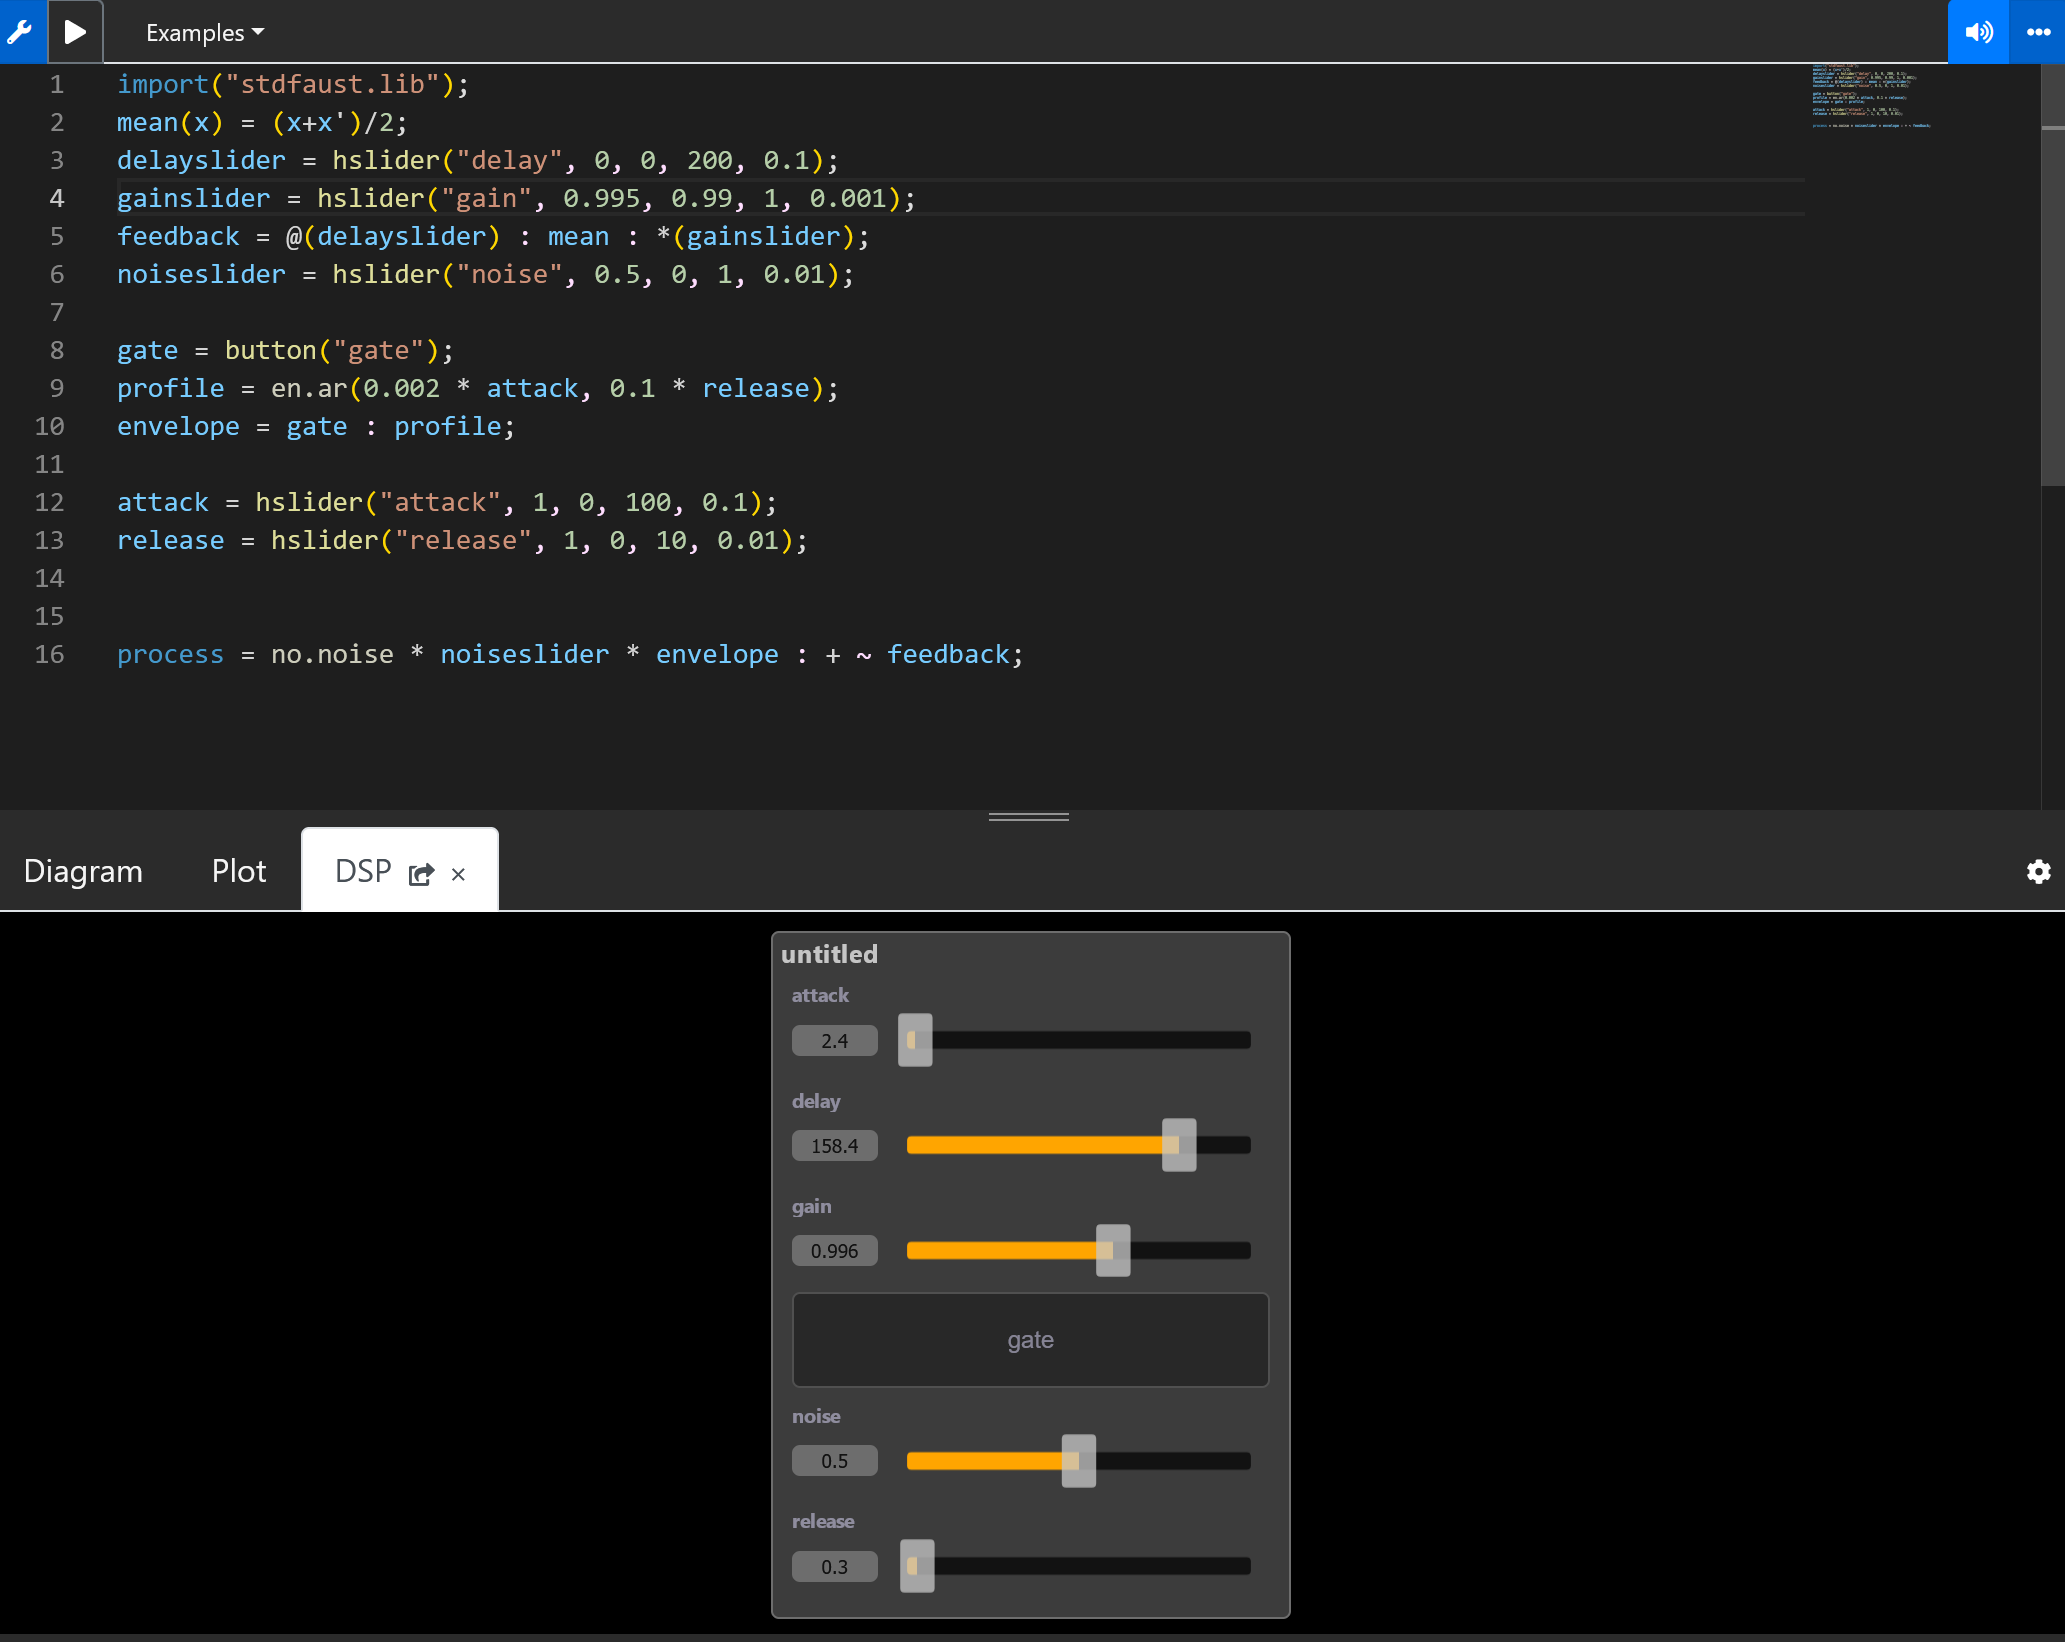
\includegraphics[width=0.8\textwidth]{imgs/guitare.png}
    \caption{Réglages pour la synthèse d'une guitare}
    \label{fig:guitar}
\end{figure}

\end{document}
